\chapter{Evaluation}
\label{chap:evaluation}

This chapter presents a detailed description of the evaluation of the alternatives, which are the combination of native Android and native iOS, Apache Cordova and Motorola Rhodes. The chapter is structured as outlined in section \ref{sec:evaluation-method}: first, the weights of the criteria are calculated; second, the weights of the alternatives are calculate and last, a cost-benefit analysis is performed.

\section{Weighting the evaluation criteria}

Because developers and architects do not necessarily share the same opinions about the evaluation criteria, the ranking of the alternatives could be different as well. Therefore, this evaluation covers these two perspectives separately and the results for both perspectives are compared in the end. Both the developer and the architect were asked to fill in a questionnaire containing all necessary pairwise comparisons (see Appendix \ref{app:questionnaire}). 

The questioned people are the same people from the interviews earlier (see section \ref{sec:interviews}) and the results of the questionnaire are illustrated in \tref{tab:l1}, \tref{tab:portability}, \tref{tab:ae}, \tref{tab:productivity}, \tref{tab:ni}, \tref{tab:ui}.

\begin{table}[h!]
    \begin{center}
        \begin{tabular}{lcccl}
            \hline
            \textbf{Architect}     & Portability & App. Experience & Productivity & Priority vector \\ 
            \hline
            Portability            & $1$         & $1/3$           & $1/5$        & $0.1047$        \\
            App. Experience        & $3$         & $1$             & $5$          & $0.6370$        \\
            Productivity           & $5$         & $1/5$           & $1$          & $0.2583$        \\
            \hline
            \multicolumn{5}{r}{$\lambda_{max} = 3.5206$, $CI = 0.2603$, $RI = 0.58$, $CR = 0.4488$} \\
            \hline
        \end{tabular}
        \\\vspace{1em}
        \begin{tabular}{lcccl}
            \hline
            \textbf{Developer}     & Portability & App. Experience & Productivity & Priority vector \\ 
            \hline
            Portability            & $1$         & $1/7$           & $1/5$        & $0.0719$        \\
            App. Experience        & $7$         & $1$             & $3$          & $0.6491$        \\
            Productivity           & $5$         & $1/3$           & $1$          & $0.2790$        \\
            \hline
            \multicolumn{5}{r}{$\lambda_{max} = 3.0649$, $CI = 0.0324$, $RI = 0.58$, $CR = 0.0559$} \\
            \hline
        \end{tabular}
        \caption{Pairwise comparison matrix for the top level of the decision tree.}
        \label{tab:l1}
    \end{center}
\end{table}

The weights for the top level criteria are virtually the same for both the architect and the developer perspective. \tref{tab:portability} also reveals a high inconsistency in the architect's judgement ($CR > 0.1$). Analysis of the judgements shows that there is no loop, i.e. there is no chain $A, B, C$ such that $A$ is more important than $B$, $B$ is more important than $C$ and $C$ is more important than $A$. However, the judgement of portability vs. application experience does not reflect the judgement of application experience vs. productivity and the judgement of productivity vs. portability since $1/3 \not = 1/5 \times 1/5$. The inconsistency ratio for the judgement of the developer is acceptable as it is below 10\%.

\TODO{Ask for a better judgement?}

\begin{table}[h!]
    \begin{center}
        \begin{tabular}{lcccl}
            \hline
            \textbf{Architect}     & Platform support & Toolset reuse & Code reuse & Priority vector \\ 
            \hline
            Platform support         & $1$            & $1/3$         & $1/7$      & $0.0918$        \\
            Toolset reuse          & $3$            & $1$           & $5$        & $0.6248$        \\
            Code reuse             & $7$            & $1/5$         & $1$        & $0.2834$        \\
            \hline
            \multicolumn{5}{r}{$\lambda_{max} = 3.7089$, $CI = 0.2545$, $RI = 0.58$, $CR = 0.6112$}\\
            \hline
        \end{tabular}
        \\\vspace{1em}
        \begin{tabular}{lcccl}
            \hline
            \textbf{Developer}     & Platform support & Toolset reuse & Code reuse & Priority vector \\ 
            \hline
            Platform support         & $1$            & $1/5$         & $1/5$      & $0.0909\ldots$  \\
            Toolset reuse          & $5$            & $1$           & $1$        & $0.4545\ldots$  \\
            Code reuse             & $5$            & $1$           & $1$        & $0.4545\ldots$  \\
            \hline
            \multicolumn{5}{r}{$\lambda_{max} = 3$, $CI = 0$, $RI = 0.58$, $CR = 0$}               \\
            \hline
        \end{tabular}
        \caption{Pairwise comparison matrix for the category ``portability''.}
        \label{tab:portability}
    \end{center}
\end{table}

In the portability category (see \tref{tab:portability}), the differences between developer and architect are more pronounced. Just like before, the judgement of the architect shows a notable amount of inconsistency. Again, there is no loop but the comparison data violates the consistency property.

\TODO{Ask for better judgement?}

\begin{table}[h!]
    \begin{center}
        \begin{tabular}{lcccl}
            \hline
            \textbf{Architect}     & Native int. & UI capabilities & Performance & Priority vector \\ 
            \hline
            Native int.            & $1$         & $1$             & $3$         & $0.4600$        \\
            UI capabilities        & $1$         & $1$             & $1/3$       & $0.2211$        \\
            Performance            & $1/3$       & $3$             & $1$         & $0.3189$        \\
            \hline
            \multicolumn{5}{r}{$\lambda_{max} = 3.5608$, $CI = 0.2804$, $RI = 0.58$, $CR = 0.4835$}\\
            \hline
        \end{tabular}
        \\\vspace{1em}
        \begin{tabular}{lcccl}
            \hline
            \textbf{Developer}     & Native int. & UI capabilities & Performance & Priority vector \\ 
            \hline
            Native int.            & $1$         & $1$             & $1/5$       & $0.1428$        \\
            UI capabilities        & $1$         & $1$             & $1/5$       & $0.1428$        \\
            Performance            & $5$         & $5$             & $1$         & $0.7142$        \\
            \hline
            \multicolumn{5}{r}{$\lambda_{max} = 3$, $CI = 0$, $RI = 0.58$, $CR = 0$}               \\
            \hline
        \end{tabular}
        \caption{Pairwise comparison matrix for the category ``Application Experience''.}
        \label{tab:ae}
    \end{center}
\end{table}

\begin{table}[h!]
    \begin{center}
        \begin{tabular}{lccl}
            \hline
            \textbf{Architect}     & Access to HW & Platform-specific svc. & Priority vector \\
            \hline
            Access to HW           & $1$          & $1/3$                  & $0.2500$        \\
            Platform-specific svc. & $3$          & $1$                    & $0.7500$        \\
            \hline
            \multicolumn{4}{r}{$\lambda_{max} = 2$, $CI = 0$, $RI = 0$, $CR = 0$}            \\
            \hline
        \end{tabular}
        \\\vspace{1em}
        \begin{tabular}{lccl}
            \hline
            \textbf{Developer}     & Access to HW & Platform-specific svc. & Priority vector \\
            \hline
            Access to HW           & $1$          & $5$                    & $0.8333\ldots$  \\
            Platform-specific svc. & $1/5$        & $1$                    & $0.1666\ldots$  \\
            \hline
            \multicolumn{4}{r}{$\lambda_{max} = 2$, $CI = 0$, $RI = 0$, $CR = 0$}            \\
            \hline
        \end{tabular}
        \caption{Pairwise comparison matrix for the category ``Native integration'' within the category ``Application Experience''.}
        \label{tab:ni}
    \end{center}
\end{table}

\begin{table}[h!]
    \begin{center}
        \begin{tabular}{lccl}
            \hline
            \textbf{Architect}  & Native L\& F & UI el. capabilities & Priority vector \\
            \hline
            Native L\& F        & $1$          & $5$                 & $0.8333\ldots$  \\
            UI el. capabilities & $1/5$        & $1$                 & $0.1666\ldots$  \\
            \hline
            \multicolumn{4}{r}{$\lambda_{max} = 2$, $CI = 0$, $RI = 0$, $CR = 0$}      \\
            \hline
        \end{tabular}
        \\\vspace{1em}
        \begin{tabular}{lccl}
            \hline
            \textbf{Developer}  & Native L\& F & UI el. capabilities & Priority vector \\
            \hline
            Native L\& F        & $1$          & $1/5$               & $0.1666\ldots$  \\
            UI el. capabilities & $5$          & $1$                 & $0.8333\ldots$  \\
            \hline
            \multicolumn{4}{r}{$\lambda_{max} = 2$, $CI = 0$, $RI = 0$, $CR = 0$}      \\
            \hline
        \end{tabular}
        \caption{Pairwise comparison matrix for the category ``UI capabilities'' within the category ``Application Experience''.}
        \label{tab:ui}
    \end{center}
\end{table}

\begin{table}[h!]
    \begin{center}
        \begin{tabular}{lcccl}
            \hline
            \textbf{Architect} & Skill reuse & Tooling & Testing & Priority vector \\
            \hline
            Skill reuse        & $1$         & $1/5$   & $3$     & $0.2021$        \\
            Tooling            & $5$         & $1$     & $5$     & $0.7007$        \\
            Testing            & $1/3$       & $1/5$   & $1$     & $0.0972$        \\
            \hline
            \multicolumn{5}{r}{$\lambda_{max} = 3.1356$, $CI = 0.0678$, $RI = 0.58$, $CR = 0.1169$}\\
            \hline
        \end{tabular}
        \\\vspace{1em}
        \begin{tabular}{lcccl}
            \hline
            \textbf{Developer} & Skill reuse & Tooling & Testing & Priority vector \\
            \hline
            Skill reuse        & $1$         & $1$     & $3$     & $0.4286$        \\
            Tooling            & $1$         & $1$     & $3$     & $0.4286$        \\
            Testing            & $1/3$       & $1/3$   & $1$     & $0.1428$        \\
            \hline
            \multicolumn{5}{r}{$\lambda_{max} = 3$, $CI = 0$, $RI = 0.58$, $CR = 0$}               \\
            \hline
        \end{tabular}
        \caption{Pairwise comparison matrix for the category ``Productivity''.}
        \label{tab:productivity}
    \end{center}
\end{table}




\section{Evaluate the alternatives}

In the subsections to follow, all alternatives get evaluated with respect to one criterion at a time. In every subsection, a description is given of what exactly is measured and how. The description also outlines what is taken into account for the evaluation, which scale is used and why. For every alternative, a rationale for the judgement or score is provided as well.

For some criteria, there is no absolute scale available to measure said property. In that case, judgements based on pairwise comparison, as proposed by Saaty \cite{Saaty:1980}, are used to evaluate the alternatives. These judgements arise from the experience of developing the proof-of-concept application. In addition, some criteria deal with features that are not addressed in the proof-of-concept application. In that case, the evaluation is based on the information that is found in the documentation. 

\TODO{Make sure every section clearly mentions these things...}

\subsection{Platform support}

Remember from section \ref{sec:selection-criteria} that support for Android and iOS is a selection criterion. This criterion only covers additional platforms, apart from Android and iOS. To reflect the value of each platform, every alternative is awarded the additional market share it can serve. In the end, these scores are normalized such that the sum of scores is equal to 1. The market share numbers are taken from \fref{fig:smartphone-share}.

\paragraph{Android \& iOS} Native code for Android and iOS is useless on other platforms. Hence, the combination of Android and iOS cannot contribute to reaching additional market share.

\paragraph{Apache Cordova} From Cordova's platform support (see section \ref{sec:ac:support}), it is safe to say that it supports the remainder of the mobile market. Cordova is therefore awarded the remaining 17\% of market share: 6\% for BlackBerry, 6\% for Symbian, 2\% for Windows Phone, 2\% for Bada and 1\% for the remainder of mobile platforms.

\paragraph{Motorola Rhodes} Rhodes only supports BlackBerry and Windows Phone for which it is awarded 8\% of market share: 6\% for BlackBerry and 2\% for Windows Phone. 

\paragraph{Verdict} The normalized scores are listed in \tref{tab:ps}. 

\begin{table}[h!]
    \begin{center}
        \begin{tabular}{lcccl}
            \hline
            \textbf{Platform support} & Market share & Normalized weight \\
            \hline
            Android/iOS               & $0\%$        & $0$         \\
            Cordova                   & $17\%$       & $0.68$      \\
            Rhodes                    & $8\%$        & $0.32$      \\
            \hline
        \end{tabular}
        \caption{Evaluation of the alternatives with respect to ``platform support''.}
        \label{tab:ps}
    \end{center}
\end{table}

\subsection{Toolset reuse}

This criterion describes the ability to reuse the development environment or parts thereof when migrating to another cross-platform alternative. The evaluation is based on the recommended development environment setup for each alternative. Since there is no absolute scale available to measure this property, Saaty's fundamental scale (see \tref{tab:ahp-scale}) is used here.

\paragraph{Android \& iOS} All iOS development is done with the Xcode IDE, which is available on Apple computers only. Every iOS developer must therefore have a rather expensive Mac. For Android development, any platform can be used in combination with the Android SDK and an Eclipse plugin (ADT) is available. On I/O 2013, Google also announced a new, freely available Android IDE, based on JetBrains' IntelliJ.

\paragraph{Apache Cordova} For HTML5 application development, any operating system with a web IDE or even a simple text editor will do. However, packaging the Cordova application in its native shell requires the native SDK's or the online build service, called PhoneGap Build, provided by Adobe. Unfortunately, this service cannot build additional plugins that are not part of the standard distribution. If a project makes use of custom plugins, the native SDK's are required. 

\paragraph{Motorola Rhodes} Development of Rhodes applications requires a Ruby installation and a Ruby IDE. A specially tailored Eclipse-based Ruby IDE, called RhoStudio, is distributed as part of RhoMobile. As with Cordova, packaging the app requires the native SDK or the online build service, called RhoHub, provided by Motorola.

\paragraph{Verdict} Motorola Rhodes and Apache Cordova have similar requirements and therefore they are treated equally in the comparison. 
Native development for Android and iOS is treated as a whole. Because of the strict requirements imposed by Apple, native development scores a little less compared to Cordova and Rhodes. However, not being able to build the application locally is not very practical either, which explains the scores listed in \tref{tab:tr}.

\begin{table}[h!]
    \begin{center}
        \begin{tabular}{lcccl}
            \hline
            \textbf{Toolset reuse} & Android/iOS & Cordova & Rhodes & Priority vector \\
            \hline
            Android/iOS            & $1$         & $1/3$   & $1/3$  & $0.1428$        \\
            Cordova                & $3$         & $1$     & $1$    & $0.4286$        \\
            Rhodes                 & $3$         & $1$     & $1$    & $0.4286$        \\
            \hline
            \multicolumn{5}{r}{$\lambda_{max} = 3$, $CI = 0$, $RI = 0.58$, $CR = 0$}  \\
            \hline
        \end{tabular}
        \caption{Evaluation of the alternatives with respect to ``toolset reuse''.}
        \label{tab:tr}
    \end{center}
\end{table}

\subsection{Code reuse}
\label{sec:cr}

This criterion measures the amount of code that can be reused when migrating to another platform. For this criterion, the amount of portable code is expressed as an estimated percentage of the total amount of application code. Native extensions are not taken into account as they are not part of the application logic. They are considered to be reusable dependency which has to be coded once. 

\paragraph{Android \& iOS} As mentioned before, native code for Android and iOS is useless on other platforms but native Android code is also useless on iOS and vice versa. Hence, code reuse on Android and iOS is 0\%.

\paragraph{Apache Cordova} Code reuse is 100\% for Cordova applications because all code is shared across all platforms. Since code of native plugins are not taken into account, this does not affect the score.

Note that a large amount of code can potentially be reused in other (non-mobile) platforms. Be that as it may, it is out of the scope of this evaluation and it is not taken into account either.

\paragraph{Motorola Rhodes} Code reuse on Rhodes applications is also 100\%. It is not taken into account that Rhodes has no support for custom plugins and that its code is not as widely deployable.

\paragraph{Verdict} The scores for each alternative are normalized and listed in \tref{tab:cr}. 

\begin{table}[h!]
    \begin{center}
        \begin{tabular}{lcccl}
            \hline
            \textbf{Toolset reuse} & Code reuse & Priority vector \\
            \hline
            Android/iOS            & $0\%$       & $0$            \\
            Cordova                & $100\%$     & $0.5000$       \\
            Rhodes                 & $100\%$     & $0.5000$       \\
            \hline
        \end{tabular}
        \caption{Evaluation of the alternatives with respect to ``code reuse''.}
        \label{tab:cr}
    \end{center}
\end{table}

\subsection{Access to hardware}

This criterion measures the ability to integrate the device's hardware. For this criterion, the availability of device API's (sensor API's, output API's and communication API's) is studied and every alternative is awarded the fraction of device API's it supports. Alternatives can either provide full support (there is a way to access a particular piece of hardware or software on both platforms), partial support (access to this type of hardware is available on one platform only) or no support. Note that most of these API's are not used in the proof-of-concept application. Therefore, this comparison is mostly based on the documentation of the alternatives.

\paragraph{Android \& iOS} Android provides support for all types of sensors but that does not imply that all these sensors are available in a particular device. Apple iDevices have less sensors and as such there is no support for every sensor in iOS.

\paragraph{Apache Cordova} Cordova tries to promote the web as a first-class platform for mobile applications. ``The ultimate purpose of \emph{Cordova} is to cease to exist'' \cite{LeRoux:2012}. When HTML5 will be fully supported on all mobile browsers, Cordova will no longer be needed. Therefore, all Cordova API's (try to) follow the HTML5 specification and do not provide support for all the sensors and communication because they are simply not in the specification.

Note that with Cordova's plugin system, it can deliver the same level of integration as native Android and iOS. However, the plugin system is not taken into account here. 

\paragraph{Motorola Rhodes} Rhodes provides a reasonable amount device API's. All of them are available through ruby method calls. As of version 3.3.3, Motorola has removed a lot of API's and included them in their commercial product called RhoMobile Suite, for which additional API's are available.

\paragraph{Verdict} The studied device API's and the alternative's support for it are listed in \tref{tab:apis}.

\begin{table}[h]
    \begin{center}
        \begin{tabular}{lcccc}
            \hline
            API                 & Android        & iOS        & Cordova    & Rhodes     \\
            \hline
            Accelerometer       & \checkmark     & \checkmark & \checkmark & \checkmark \\
            Geolocation         & \checkmark     & \checkmark & \checkmark & \checkmark \\
            Gyroscope           & \checkmark     & \checkmark & --         & \checkmark \\
            Light               & \checkmark     & \checkmark & --         & \checkmark \\
            Magnetic Field      & \checkmark     & \checkmark & \checkmark & \checkmark \\
            Pressure            & \checkmark     & --         & --         & partial    \\
            Proximity           & \checkmark     & \checkmark & --         & \checkmark \\
            Relative Humidity   & \checkmark     & --         & --         & partial    \\
            Temperature         & \checkmark     & --         & --         & partial    \\
            Microphone          & \checkmark     & \checkmark & \checkmark & \checkmark \\
            Camera              & \checkmark     & \checkmark & \checkmark & \checkmark \\
            Hardware buttons    & \checkmark     & --         & partial    & partial    \\
            Vibration Motor     & \checkmark     & \checkmark & \checkmark & partial    \\
            Speaker             & \checkmark     & \checkmark & \checkmark & \checkmark \\
            System information  & \checkmark     & \checkmark & \checkmark & \checkmark \\
            File System         & \checkmark     & \checkmark & \checkmark & \checkmark \\
            Contacts            & \checkmark     & \checkmark & \checkmark & \checkmark \\
            Bluetooth           & \checkmark     & \checkmark & --         & \checkmark \\
            NFC                 & \checkmark     & --         & --         & --         \\
            Wi-Fi Direct        & \checkmark     & --         & --         & --         \\
            USB / Accessory     & \checkmark     & \checkmark & --         & --         \\
            \hline
            Support             & \multicolumn{2}{c}{Average: $18/21$} & $10.5/21$  & $15.5/21$  \\
            \hline
        \end{tabular}
        \caption{Evaluation of the alternatives with respect to ``access to hardware''.}
        \label{tab:apis}
    \end{center}
\end{table}

\subsection{Integration with platform-specific services}

This criterion measures the ability of an alternative to integrate the application with platform-specific services that might not be available on all platforms, e.g. Passbook. The proof-of-concept application does not contain this kind of integration and consequently this evaluation is based on the documentation. Because there is no absolute scale to quantify this property, the evaluation is also based on judgements.

\paragraph{Android \& iOS} Platform-specific services are part of the native SDK's. Therefore, this kind of integration is implemented the easiest in the native applications.

\paragraph{Apache Cordova} There are no API's for this kind of integration in the default distribution but fortunately, Cordova ships with an elaborate plugin-system which can be used to deal with it.

\paragraph{Motorola Rhodes} There are no API's for this integration in Rhodes either. Moreover, Rhodes does not have a plugin system which could make this integration possible. Therefore, it is excluded from this category and not awarded any points.

\paragraph{Verdict} The scores are listed in \tref{tab:pss}. Integrating with platform specific services is clearly more easy with the native development kits.

\begin{table}[h!]
    \begin{center}
        \begin{tabular}{lcccl}
            \hline
            \textbf{Performance} & Android/iOS & Cordova & Rhodes & Priority vector \\
            \hline
            Android/iOS          & $1$         & $5$     & excl. & $0.8333\ldots$        \\
            Cordova              & $1/5$       & $1$     & excl. & $0.1667\ldots$        \\
            Rhodes               & excl.       & excl.   & excl. & $0$        \\
            \hline
            \multicolumn{5}{r}{$\lambda_{max} = 2$, $CI = 0$, $RI = 0$, $CR = 0$}\\
            \hline
        \end{tabular}
        \caption{Evaluation of the alternatives with respect to ``platform-specific services''}
        \label{tab:pss}
    \end{center}
\end{table}

\subsection{Native Look \& Feel}

This criterion indicates whether or not an alternative is able to use native user interface elements. An application can either support the use of native user interface elements fully, partially or not at all.

\paragraph{Android \& iOS} It needs no explaining that Android and iOS can use the native user interface elements.

\paragraph{Apache Cordova} The user interface of Cordova applications is built with HTML5, CSS and JavaScript and there is no possibility to use native user interface elements for it. 

However, numerous attempts are made to recreate the native look \& feel on top of HTML (like KendoUI, Moobile, etc.). Unfortunately, these projects need a lot of additional code to mimic the behaviour of native interface elements which influences the overall performance of the application in a adverse way.

\paragraph{Motorola Rhodes} The user interface of Rhodes applications is also built with HTML and consequently cannot deliver the native look \& feel to the end user.

\paragraph{Verdict} Despite the efforts of many projects to mock the native look \& feel in web applications, it remains a privilege of Android and iOS. Hence, Android and iOS clearly do better compared to Cordova and Rhodes, as is illustrated in \tref{tab:nlf}.

\begin{table}[h!]
    \begin{center}
        \begin{tabular}{lcl}
            \hline
            \textbf{Native Look \& Feel} & Native L\&F & Priority vector \\
            \hline
            Android/iOS          & Yes      & $1$  \\
            Cordova              & No       & $0$  \\
            Rhodes               & No       & $$   \\
            \hline
        \end{tabular}
        \caption{Evaluation of the alternatives with respect to ``Native look \& feel''.}
        \label{tab:nlf}
    \end{center}
\end{table}

\subsection{UI element capabilities}

This criterion measures an alternative's potential to present a rich user interface. Both Cordova and Rhodes rely on HTML for their user interface. Therefore, the evaluation is based on a comparison of the native UI elements with their HTML5 counterparts. Plain HTML only provides basic interface elements, which is why an additional UI framework, called Bootstrap\footnote{\url{http://getbootstrap.com}}, was used to develop the proof-of-concept application. 

\paragraph{Android \& iOS} Android and iOS both have an elaborate portfolio of rich user interface elements. iOS lacks some basic form elements like radio buttons and checkboxes but these can be easily replaced with pickers and switches respectively.

\paragraph{Apache Cordova} Cordova applications are mobile web applications that are wrapped in a single webview. Hence, only HTML5 can be used to create the user interface. An application could be comprised of multiple pages or it could be comprised of a single page, in which case it is called  a single-page application. The former approach requires page reloads, which feels unnatural in a mobile app (compared to native apps) whereas the latter approach can make the hybrid app behave more like a native app. 

The Cordova proof-of-concept application is implemented as a single-page application with AngularJS\footnote{\url{http://angularjs.org}}. This framework drastically improves productivity by reducing the required lines of code through declarative programming and bidirectional bindings between view and model. 

\paragraph{Motorola Rhodes} Rhodes also relies on HTML for its user interface. In contrast to Cordova, Rhodes is actually a complete web server with an MVC framework on top. Every request is handled locally by a controller action and the result is served in a webview. Developers can still choose to create single-page applications but device integration has to be realized through AJAX\footnote{Asynchronous JavaScript and XML} calls, which requires extra work. The proof-of-concept application is implemented as a multi-page application because this is the default way to develop applications with Rhodes.

\paragraph{Verdict} The scores are listed in \tref{tab:uiec}.

\begin{table}[h]
    \begin{center}
        \begin{tabular}{llll}
            \hline
            Android         & iOS              & HTML5                          & Bootstrap 3             \\
            \hline
            ActionBar       & UINavigationBar  & --                             & \html{navbar} class     \\
            Split ActionBar & UIToolbar        & --                             & \html{navbar} class     \\
            Tabs            & UITabBar         & --                             & \html{nav-tabs} class   \\
            ListView        & UITableView      & --                             & \html{list-group} class \\
            GridList        & UICollectionView & --                             & Grid system             \\            
            ScrollView      & UIScrollView     & by default                     & --                      \\
            Spinner         & --               & \html{<select></select>}       & \html{dropdown} class   \\
            Picker          & UIPickerView     & \html{<select></select>}       & \html{modal} class      \\
            DatePicker      & UIDatePicker     & \html{<input type="date">}     & --                      \\
            Button          & UIButton         & \html{<button></button>}       & \html{btn} class        \\
            Text field      & UITextField      & \html{<input type="...">}      & --                      \\
            Slider          & UISlider         & \html{<input type="range">}    & --                      \\
            Progress bar    & UIProgressBar    & \html{<progress>}              & \html{progress} class   \\
            Options Menu    & UIActionSheet    & --                             & --                      \\
            Checkbox        & --               & \html{<input type="checkbox">} & --                      \\
            Radio           & --               & \html{<input type="radio">}    & --                      \\
            On/off switch   & UISwitch         & --                             & \html{btn-group} class  \\
            Dialog          & UIDialog         & --                             & \html{modal} class      \\
            Alert           & UIAlertView      & \html{alert(string)}           & --                      \\
            Popup           & --               & --                             & \html{modal} class      \\
            Toast           & --               & --                             & \html{alert} class      \\
            TextView        & UILabel          & any text element               & --                      \\
            MapView         & MKMapView        & --                             & --                      \\
            --              & Popover (iPad)   & --                             & \html{popover} script   \\
            Master-Detail   & SplitView (iPad) & --                             & Grid System             \\
            WebView         & UIWebView        & \html{<iframe>}                & --                      \\
            \hline
            \multicolumn{2}{c}{Android \& iOS combined: $26/26$} & \multicolumn{2}{c}{HTML5 \& Bootstrap combined: $24/26$}                 \\
            \hline
        \end{tabular}
        \caption{Evaluation of the alternatives with respect to ``UI element capabilities''.}
        \label{tab:uiec}
    \end{center}
\end{table}


\subsection{Performance}

The performance criterion measures the responsiveness of the user interface and the application in general. Responsiveness in this case does not mean the ability to reflow UI elements to fit other screen sizes, responsiveness in this case represents the time it takes an application to respond to a trigger, like pushing a button.

Comparing the performance of these alternatives is hard because their architectures are completely different. For web applications, page load times could be a viable metric. However, only the Rhodes application uses page loads. There is no notion of page loads in native applications and the Cordova application is implemented as a single-page application. Hence, no absolute scale is available and the alternatives are evaluated based on judgement. The analytic hierarchy process can deal with inconsistency as long as the consistency ratio is low, i.e equal or below 10\%. In that case, the judgements are accepted.

Every implementation of the proof-of-concept application is tested on four devices:
\begin{itemize}
    \item \textbf{HTC Wildfire S} An entry-level smartphone, released in May 2011 and running Android 2.3.5 on a single core 600\,MHz ARMv6 processor. It has 512\,MB of RAM and a 3.2-inch display with a 320 by 480 pixel resolution (180\,ppi).
    \item \textbf{HTC Flyer} An entry-level tablet, also released in May 2011 and running Android 3.2.2 on a single core 1.5\,GHz ARMv7 processor. It has 1024\,MB of RAM and a 7.0-inch display with a 600 by 1024 pixel resolution (170\,ppi).
    \item \textbf{LG/Google Nexus 4} A high-end smartphone, released in November 2012 and running Android 4.2.2 on a quad core 1.5\,GHz ARMv7 processor. It has 2048\,MB of RAM and a 4.7-inch display with a 768 by 1280 pixel resolution (318\,ppi).
    \item \textbf{iPhone 3GS} A smartphone, released in June 2009 and running iOS 6.1.3 on a single core 600\,MHz ARMv6 processor. It has 256\,MB of RAM and a 3.5-inch display with a 320 by 480 pixel resolution (165\,ppi).
\end{itemize}

\paragraph{Android \& iOS} The native SDK's are the most suited to take advantage of the device capabilities. Therefore, native applications always perform the best, provided they are well-designed.

\paragraph{Apache Cordova} Cordova wraps web applications. Hence, the performance of its applications greatly depends on the performance of the browser on the device. On older smartphones, the performance of the browser is often seriously lacking. The use of a single-page application solves this issue in a way, but the performance drop is still notable.

\paragraph{Motorola Rhodes} A Rhodes application also relies on the native browser to display its user interface. The difference with Cordova is that Rhodes uses a local ruby web server to serve multi-page applications. The performance of the local web server is absolutely disappointing, resulting in utterly slow page loads (of up to 30 seconds for a single load on the slowest devices and 7 seconds on the fastest device).

\paragraph{Verdict} The judgements for this evaluation are listed in \tref{tab:performance}. The consistency ratio is rather high but still acceptable.

\begin{table}[h!]
    \begin{center}
        \begin{tabular}{lcccl}
            \hline
            \textbf{Performance} & Android/iOS & Cordova & Rhodes & Priority vector \\
            \hline
            Android/iOS          & $1$         & $5$     & $9$    & $0.7352$        \\
            Cordova              & $1/5$       & $1$     & $5$    & $0.2067$        \\
            Rhodes               & $1/9$       & $1/5$   & $1$    & $0.0581$        \\
            \hline
            \multicolumn{5}{r}{$\lambda_{max} = 3$, $CI = 0.0585$, $RI = 0.58$, $CR = 0.10$}\\
            \hline
        \end{tabular}
        \caption{Evaluation of the alternatives with respect to ``Performance''.}
        \label{tab:performance}
    \end{center}
\end{table}

\subsection{Skill reuse}

This criterion expresses the ability to reuse skills from another field of expertise to develop mobile applications. This allows for better resource management. For this criterion, it is assumed that the organization has got a substantial expertise with Java EE (because Capgemini does). 

\paragraph{Android \& iOS} For organizations that already have got  expertise with Java EE applications, the entry barrier for adding Android to the portfolio is rather low, since Android is based on Java. Adding iOS from that perspective is less straightforward, because Objective-C is a new programming language.

\paragraph{Apache Cordova} In order to develop Cordova applications, one needs to know the web. Since the web already belongs to the organization's expertise, this skill can be reused quite easily but developers will probably have to invest in their JavaScript skills. When custom plugins are needed, the scenario of native Android and iOS holds.

\paragraph{Motorola Rhodes} For Rhodes applications, organizations can reuse their skills for creating the user interface. However, the application logic entirely written in Ruby, which is a new programming language for the organization.

\paragraph{Verdict} The native SDK's and Rhodes are similar because one needs to learn a new language for either of both. For the development of Cordova application, no notable new skills are required, explaining the scores listed in \tref{tab:sr}.

\TODO{On the other hand, learning Objective-C appeared to be easier than learning Ruby (in combination with Rhodes) when developing the proof-of-concept application. The free online video lectures about iOS development by Paul Hegarty are very valuable.}


\begin{table}[h!]
    \begin{center}
        \begin{tabular}{lcccl}
            \hline
            \textbf{Skill reuse} & Android/iOS & Cordova & Rhodes & Priority vector \\
            \hline
            Android/iOS          & $1$         & $1/5$   & $1/5$  & $0.1428$        \\
            Cordova              & $5$         & $1$     & $5$    & $0.7144$        \\
            Rhodes               & $1$         & $1/5$   & $1$    & $0.1428$        \\
            \hline
            \multicolumn{5}{r}{$\lambda_{max} = 3$, $CI = 0$, $RI = 0.58$, $CR = 0$}\\
            \hline
        \end{tabular}
        \caption{Evaluation of the alternatives with respect to ``Skill reuse''.}
        \label{tab:sr}
    \end{center}
\end{table}

\subsection{Tooling}

This criterion describes the overall quality of the supplied tools. This includes command-line interfaces, IDE's, emulators and others. Since there is no absolute scale available to measure the quality accurately, the alternatives are compared in pairs. Saaty's scale is used to express the scores that are based on the experience of developing the proof-of-concept application.

\paragraph{Android \& iOS} The restrictions on Apple development may seem obstructive at first but it also allows Apple to deliver a well integrated development environment. Everything a developer could possibly need is available in Xcode, right out of the box. For Android development, an Eclipse plugin is available which integrates all the functionality of the SDK with the IDE. 

\paragraph{Apache Cordova} Cordova does not ship with an elaborate IDE or special development tools. However, there are some tools that can ease the development of mobile web applications (WEINRE, Ripple emulator, etc.). Unfortunately, there is no integrated development environment. 

\paragraph{Motorola Rhodes} Rhodes comes with a bunch of command-line scripts. Sadly, the Android Debug Bridge (ADB) is poorly integrated \TODO{(see section \ref{sec:mr:tools})} and there is no option to transfer iOS applications to an iDevice from the command-line interface. Instead, either Xcode, iTunes or Fruitstrap is needed for the transfer. 

\TODO{What about RhoStudio?}

\paragraph{Verdict} The scores about the quality of the tools are based on the experience from developing the proof-of-concept application and are listed in \tref{tab:tooling}. 

\begin{table}[h!]
    \begin{center}
        \begin{tabular}{lcccl}
            \hline
            \textbf{Tooling} & Android/iOS & Cordova & Rhodes & Priority vector \\
            \hline
            Android/iOS      & $1$         & $3$     & $9$    & $0.6716$        \\
            Cordova          & $1/3$       & $1$     & $5$    & $0.2654$        \\
            Rhodes           & $1/9$       & $1/5$   & $1$    & $0.0629$        \\
            \hline
            \multicolumn{5}{r}{$\lambda_{max} = 3$, $CI = 0.0145$, $RI = 0.58$, $CR = 0.025$}\\
            \hline
        \end{tabular}
        \caption{Evaluation of the alternatives with respect to ``Tooling''.}
        \label{tab:tooling}
    \end{center}
\end{table}

\subsection{Testing}

This criterion measures the ability to (1) write tests and (2) automate testing in a continuous integration environment. This criterion focusses mainly on unit testing and integration testing as these tests are most common. Mobile interface testing is rather hard and is not taken into account for this criterion. Alternatives are evaluated using judgements because there is no absolute scale on which this property could be quantified. 

Continuous integration is actually not part of the scope for the proof-of-concept application. Nevertheless, this is an important topic in a production environment and therefore it is examined superficially.

\paragraph{Android \& iOS} Android and iOS have built-in support for writing unit tests (1). Android is based on Java and consequently, the well-known JUnit framework can be used for writing tests. For iOS, a similar framework is readily available in Xcode for Objective-C. 

For automated testing in a continuous integration environment (2), there are a number of options available. Continuous integration testing for Android can be set up quite easily with Jenkins\footnote{Jenkins is a popular continuous integration server, \url{http://jenkins-ci.org}}, even headless\footnote{On a server without a user interface}. For iOS, there are a number of guides available describing how to set it up. However, a Apple hardware is still required. Other options include a hosted continuous integration service.

\paragraph{Apache Cordova} For JavaScript, the Jasmine testing framework\footnote{\url{http://pivotal.github.io/jasmine/}} can be used to write tests (1). In combination with a test runner like Karma\footnote{\url{http://karma-runner.github.io/0.8/index.html}}, these test can be ran in a continuous integration environment. Better yet, this framework allows to automate testing on the actual mobile devices.

\paragraph{Motorola Rhodes} Unit testing is also built-in into Rhodes. However, only few options seem to be available for automating testing in a continuous integration environment.

\paragraph{Verdict}  The judgements are summarized in \tref{tab:testing}. All alternatives have support for unit testing. In that perspective, they are all equal. Rhodes seems to be less suited for continuous integration when compared to the other alternatives. The other alternatives perform equally because seem to support the same features.

\begin{table}[h!]
    \begin{center}
        \begin{tabular}{lcccl}
            \hline
            \textbf{Testing} & Android/iOS & Cordova & Rhodes & Priority vector \\
            \hline
            Android/iOS      & $1$         & $1$     & $3$    & $0.4286$ \\
            Cordova          & $1$         & $1$     & $3$    & $0.4286$ \\
            Rhodes           & $1/3$       & $1/3$   & $1$    & $0.1428$ \\
            \hline
            \multicolumn{5}{r}{$\lambda_{max} = 3$, $CI = 0$, $RI = 0.58$, $CR = 0$}\\
            \hline
        \end{tabular}
        \caption{Evaluation of the alternatives with respect to ``Testing''.}
        \label{tab:testing}
    \end{center}
\end{table}

\subsection*{Global verdict}

With the information from the evaluation above, the total weight $a_j$ of every alternative $A_j$ is calculated as
\begin{gather}
    a_j = \sum_{i = 0}^{m} c_i w_i \quad j = 1, \ldots, n
\end{gather}
where $c_i$ is the weight of the criterion $C_i$ and $w_i$ is the weight of alternative $A_j$ with respect to criterion $C_i$. The total weights are calculated for both the architect and developer and are listed in \tref{tab:total:architect} and \tref{tab:total:developer} respectively. 

\begin{table}[h]
    \begin{center}
        \begin{tabular}{lcccc}
            \hline
            \textbf{Architect}         & $c_i$    & $c_i w_{Android/iOS}$ & $c_i w_{Cordova}$  & $c_i w_{Rhodes}$ \\
            \hline
            Platform support           & $0.0096$ & $0.0000$              & $0.0065$           & $0.0031$     \\
            Toolset reuse              & $0.0654$ & $0.0093$              & $0.0280$           & $0.0280$     \\
            Code reuse                 & $0.0297$ & $0.0000$              & $0.0148$           & $0.0148$     \\
            Access to hardware         & $0.0733$ & $0.0300$              & $0.0175$           & $0.0258$     \\
            Platform-specific services & $0.2198$ & $0.1831$              & $0.0366$           & $0.0000$     \\
            Native Look \& Feel        & $0.1174$ & $0.1174$              & $0.0000$           & $0.0000$     \\
            UI element capabilities    & $0.0235$ & $0.0110$              & $0.0062$           & $0.0062$     \\
            Performance                & $0.2031$ & $0.1493$              & $0.0420$           & $0.0118$     \\
            Skill reuse                & $0.0522$ & $0.0135$              & $0.0333$           & $0.0055$     \\
            Tooling                    & $0.1810$ & $0.1216$              & $0.0480$           & $0.0114$     \\
            Testing                    & $0.0251$ & $0.0108$              & $0.0108$           & $0.0036$     \\
            \hline
            $a_j$                      &          & $0.6460$              & $0.2438$           & $0.1328$     \\
            \hline
        \end{tabular}
        \caption{Summary of the total weight and weighted scores of the alternatives with respect to the architect's weights.}
        \label{tab:total:architect}
    \end{center}
\end{table}

\begin{table}[h]
    \begin{center}
        \begin{tabular}{lcccc}
            \hline
            \textbf{Architect}         & $c_i$        & $c_i w_{Android/iOS}$ & $c_i w_{Cordova}$  & $c_i w_{Rhodes}$ \\
            \hline
            Platform support           & $0.0065$     & $0.0000$          & $0.0044$       & $0.0021$     \\
            Toolset reuse              & $0.0327$     & $0.0047$          & $0.0140$       & $0.0140$     \\
            Code reuse                 & $0.0327$     & $0.0000$          & $0.0163$       & $0.0163$     \\
            Access to hardware         & $0.0772$     & $0.0316$          & $0.0184$       & $0.0272$     \\
            Platform-specific services & $0.0155$     & $0.0129$          & $0.0026$       & $0.0000$     \\
            Native Look \& Feel        & $0.0155$     & $0.0155$          & $0.0000$       & $0.0000$     \\
            UI element capabilities    & $0.0772$     & $0.0363$          & $0.0205$       & $0.0205$     \\
            Performance                & $0.4636$     & $0.3408$          & $0.0958$       & $0.0269$     \\
            Skill reuse                & $0.1196$     & $0.0309$          & $0.0762$       & $0.0125$     \\
            Tooling                    & $0.1196$     & $0.0803$          & $0.0317$       & $0.0075$     \\
            Testing                    & $0.0398$     & $0.0171$          & $0.0171$       & $0.0057$     \\
            \hline
            $a_j$                      &              & $0.5700$          & $0.2971$       & $0.1328$     \\
            \hline
        \end{tabular}
        \caption{Summary of the total weight and weighted scores of the alternatives with respect to the developer's weights.}
        \label{tab:total:developer}
    \end{center}
\end{table}

The ranking of the alternatives is the same for both. Conversely, the average total weight can be calculated without changing the order. Android and iOS clearly offer the most benefits with an average total weight of 60.80\%. Cordova comes second with an average total weight of 27.04\%. Rhodes finishes last with an average total weight of 12.15\%. 

When comparing the alternatives in pairs and using Saaty's scale (see \tref{tab:ahp-scale}), one can conclude that:
\begin{itemize}
    \item Android and iOS are a little better than Cordova ($60.8/27.04 = 2.25$),
    \item Android and iOS are a little better than Cordova ($60.8 / 12.15 = 5$) and
    \item Cordova is a little better than Rhodes ($27.04 / 12.15 = 2.22$).
\end{itemize}

\section{Costs versus benefits}

Having the most benefits does not imply that a tool is the most cost-effective. No company should waste their resources on a cross-platform tool that is not profitable. Benefits and costs are deliberately separated from the beginning to allow the decision maker to make a cost-benefit analysis. In this section, the benefits of each alternative will be compared to their costs.

There are two types of costs. The first category, called fixed costs, are independent of the amount of produced code and includes license and subscription fees, developer tools, etc. Because these costs can be shared across projects, their impact on the total cost of a project is rather small. The second category, called variable costs, are dependent of the amount of produced code and includes for instance the rates of the people involved.

Software is essentially a collection of lines of code that is produced in a certain amount of time. This time is expressed in man-months, making abstraction of the amount of people contributing to it, i.e. 2 man-months are equal to the work of 2 individuals during 1 month. Consequently, duration is a good estimate for the total cost of a software project.

Developing natively for both Android and iOS requires about twice the time that is needed to develop the application for one platform only. This is a consequence of the impossibility to reuse code across platforms (see section \ref{sec:cr}). Developing mobile web applications for Android and iOS with Apache Cordova requires about half of the development time because 100\% of the code can be reused across platforms. The downside of this approach is that about half of the benefits are lost as well. Nevertheless, in terms of cost-effectiveness, both perform equally well. Compared to Cordova, Rhodes applications are estimated to need a little bit more work because it lacks some common but frequently used functionality (like session management). However, the benefits associated with Rhodes are considerably lower than with Cordova. These findings are visualized in \fref{fig:cost-benefit}.

\begin{figure}
    \begin{center}
        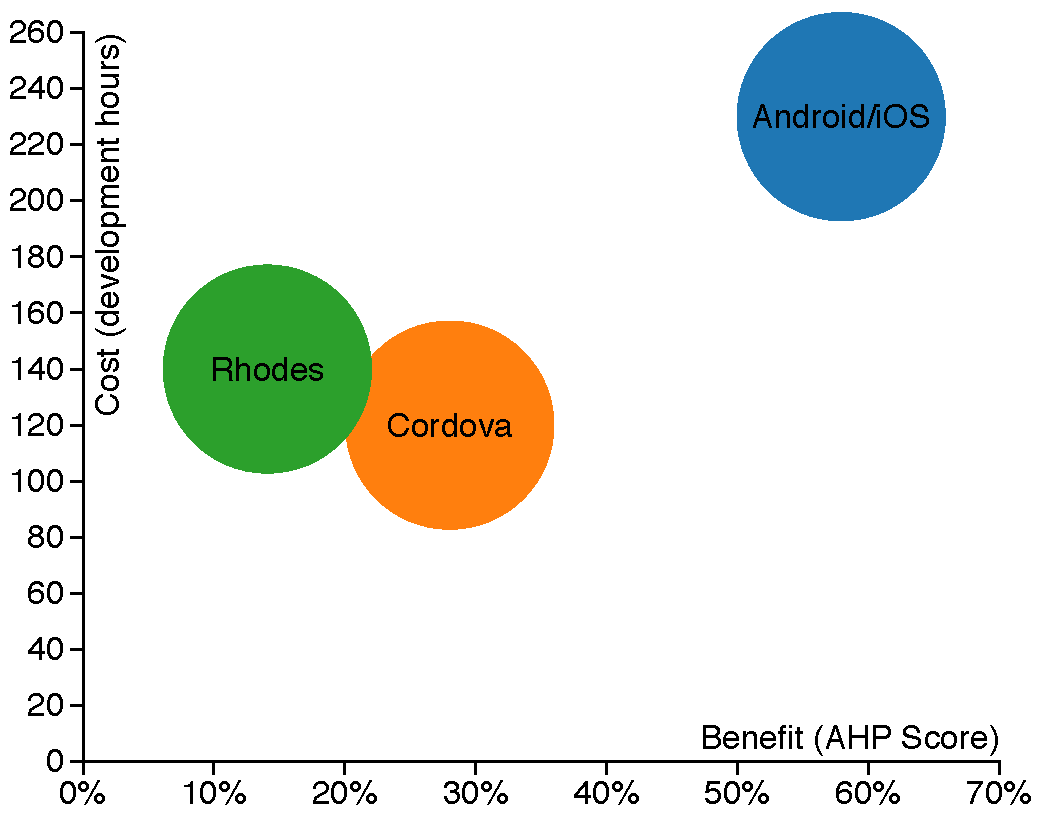
\includegraphics[width=0.7\textwidth]{figs/benefit-cost.pdf}
        \caption{Visual representation of the cost-benefit analysis.}
        \label{fig:cost-benefit}
    \end{center}
\end{figure}

Note that adding an additional platform to the native portfolio will increase the development time (and cost) by half, whereas additional platforms can be added at virtually no cost when developing mobile web applications with Cordova. In case a third platform has to be supported, Cordova application will have better value-for-money.
